\documentclass[a4paper, 11pt]{article}

\usepackage[british]{babel}
\usepackage[autostyle]{csquotes}
\usepackage[colorlinks=true, urlcolor=blue, citecolor=blue]{hyperref}
\usepackage{graphicx}
\usepackage{float}
\usepackage{geometry}
\usepackage[ruled,vlined]{algorithm2e}

\graphicspath{{images/}}
\geometry{margin=2.0cm}

\begin{document}

\title{Borůvka's Algorithm}
\author{Student Number: 690065435}
\date{December 2022}

\maketitle

% TODO: Write this at the end.
\begin{abstract}
[Abstract here.]
\end{abstract}



\vspace*{\fill}
\begin{center}
% TODO: Update this.
Word Count: 1,500

\vspace{1em}
I certify that all material in this dissertation which is not my own work has been identified.
\end{center}
\vspace{1em}

Signature: \hrulefill

\newpage
\section{Principles of Borůvka's Algorithm}
Borůvka's algorithm is a greedy algorithm that finds a minimum spanning tree for a connected, edge-weighted undirected graph. It originated from Otakar Borůvka in 1926, as a method of constructing an efficient electricity network for Moravia, a region of the Czech Republic \cite{nevsetvril2001otakar}. At the point of creation, computers as we know them today did not exist, so the algorithm was implemented by hand -- this explains why the algorithm is simpler and uses basic data structures compared to other minimum spanning tree algorithms such as Prim's and Kruskal's algorithms. Borůvka's algorithm was the first to solve the minimum spanning tree problem in polynomial time \cite{deterministicMSTs}, which was significant because it made it practical to solve the problem for large graphs and therefore more applicable to real-world problems.

It was independently rediscovered by numerous other researchers in later years, most notably by Georges Sollin in 1965, which has led to the algorithm also being known as Sollin's algorithm in parallel computing literature \cite{sollin1965trace}. 

The algorithm uses a divide-and-conquer approach that is based on the idea of building a forest of trees, and is a hybrid of Prim's and Kruskal's algorithms to find a minimum spanning tree. As aforementioned, an advantage of Borůvka's algorithm over Prim's and Kruskal's is that it does not have to pre-sort the edges, nor does it have to maintain a priority queue. In each iteration, it finds the cheapest edge that connects two different trees and combines the trees into a single tree. Borůvka's algorithm continues to iterate until there is only one tree left, which is the minimum spanning tree.

\begin{figure}[h]
    \caption{Borůvka's Short Paper \cite{nevsetvril2001otakar}}
    \begin{center}
        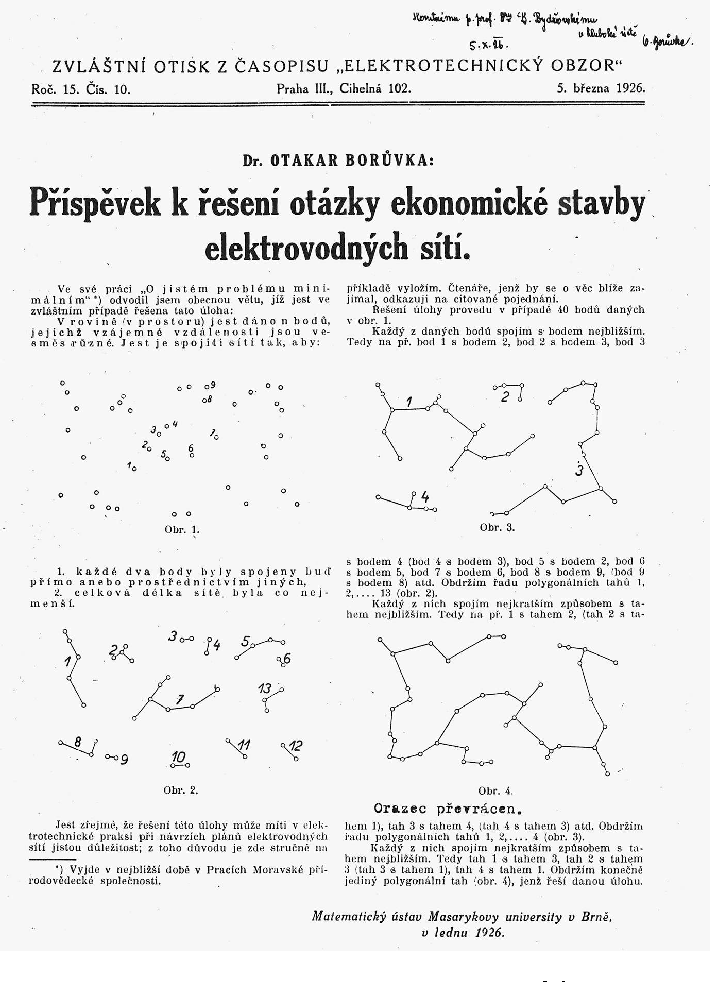
\includegraphics[width=0.6\textwidth]{Boruvka's Short Paper.png}
    \end{center}
\end{figure}

\section{Pseudocode}

% TODO: Revisit this to check whether it's correct.
\begin{algorithm}
    \caption{Borůvka's Algorithm}
    \SetKwInOut{Input}{Input}
    \SetKwInOut{Output}{Output}
    
    \Input{A connected, edge-weighted, undirected graph $G = (V, E)$}
    \Output{$T$ (a minimum spanning tree of $G$) and $totalCost$ (the total cost of $T$)}

    \nl Initialise a minimum spanning tree $T$ = (V, E'), where E' = \{\}.

    \nl Initialise the total cost of the minimum spanning tree, $totalCost = 0$.

    \nl Initialise a list of components $N$, where $N_k$ denotes the vertices in component $k$.

    \nl \For{each vertex $v$ in $V$}{
        \nl $N_v = v$.
    }

    \nl \While{$|N|$ > 1}{
        \nl Initialise an empty list of minimum connecting edges, $L$ = \{\}.

        \nl \For{each component $C$ in $N$}{
            \nl Initialise the cheapest edge $e$ to $\infty$.

            \nl \For{each edge $e'$ in $C$}{
                \nl \If{$e'$ contains an endpoint that isn't in $C$ and $e'$ is cheaper than $e$}{
                    \nl Set $e$ to $e'$.
                }
            }

            \nl \If{$e$ is not $\infty$}{
                \nl Add $e$ to $L$.
            }
        }

        \nl \For{each edge $e$ in $L$}{
            \nl \If{$e$ connects two different components}{
                \nl Merge the components $N_i$ and $N_j$ into a single component, $N_k$, such that $N_k = N_i \cup N_j$.

                \nl Add $e$ to $E'$ in $T$.

                \nl Add the edge's weight to the total cost: $totalCost = totalCost + e.weight$
            }
        }
    }

    \nl \Return $T$ and $totalCost$.
\end{algorithm}

\subsection{Flowchart}
% TODO: Add flowchart here.

\section{Time and Space Complexity Analysis}
Borůvka's algorithm has a time complexity of O(E log(V)), where E is the number of edges and V is the number of vertices in the graph.

The outer loop runs for log(V) iterations, as each iteration of the algorithm reduces the number of trees to at most half of the previous number of trees. Within each iteration, the algorithm performs a single pass over all the edges to find the minimum weight edge that connects two different components. This is performed in O(E) time, as the algorithm must consider each edge once. The algorithm then performs a single pass over all the edges to merge two components into one where possible, which is also performed in O(E) time. This gives a total time complexity of O(E log(V)).

The space complexity of Borůvka's algorithm is O(V), as it only stores the component information for each vertex, which contains each vertex's parent and minimum weight edge.

\section{Limitations and Constraints}
A limitation of Borůvka's algorithm is that it may not always find the true minimum spanning tree of a graph when the cheapest edge that connects two different components is not part of the true minimum spanning tree. This is because Borůvka's algorithm only considers the cheapest edge that connects two different components, and does not consider the cheapest edge that connects two components that are already connected. Other algorithms such as Kruskal's algorithm and Prim's algorithm do not have this limitation, as they consider all edges in the graph.

Furthermore, Borůvka's algorithm can be slow to find the minimum spanning tree when the graph has a large number of components or when the components in the graph are large in size. In these cases, the algorithm will have to perform more iterations and contract more edges.

Compared to Prim's algorithm, which runs in O(E + V log(V)) amortised time when using a Fibonacci heap \cite{fredman1987fibonacci}, Borůvka's algorithm is slightly slower. However, this variation of Prim's algorithm with the Fibonacci heap is more complicated to implement.

Borůvka's algorithm only works on undirected graphs as it does not account for the direction of the edges, thus it cannot solve the directed minimum spanning tree problem, which is more complex than the minimum spanning tree problem. Other algorithms such as the Chu-Liu/Edmonds' algorithm (originally proposed in 1965) can solve the directed minimum spanning tree problem \cite{gabow1986efficient}.

\section{Applications}
As Borůvka's algorithm finds a minimum spanning tree, it is most directly used in the design of networks, such as electrical networks, communication networks, and transportation networks \cite{graham1985history}. In the original application of an electricity network for Moravia, the vertices represented towns, and edges represented the distances between towns. Borůvka used the assumption that it was not necessary to directly connect every town to the source of electricity -- it was sufficient for a town to connect via another town that was already connected to power \cite{nevsetvril2001otakar}.

Boruvka's algorithm satisfies the triangle inequality and finds a minimum spanning tree, so it also acts as a two-approximation algorithm for the travelling salesman problem \cite{andreae1995performance}, which is NP-hard and thus not possible to solve in polynomial time \cite{junger1995traveling}. Because it produces a two-approximation, the output is at most twice the cost of the optimal solution. This can be proven as the total cost of a full walk is at most twice the cost of the minimum spanning tree, and the algorithm returns a path with a cost less than the full walk, as our pre-order walk replaces two or more edges of the full walk with a single edge \cite{andreae1995performance}.

\begin{algorithm}
    \caption{Two-Approximation for the Travelling Salesman Problem with MST-DFS \cite{andreae1995performance}}
    \nl Set a vertex as the start.
    
    \nl Construct a minimum spanning tree, $T$.
    
    \nl Create a list of vertices, $H$, that is ordered according to when they are visited in a pre-order tree walk of $T$, and add the start vertex at the end.
    
    \nl Return the path $H$.
\end{algorithm}

There are several other algorithms that are more optimal for finding a minimum spanning tree depending on the input graph -- Prim's algorithm is faster for dense graphs, and Kruskal's algorithm is faster for sparse graphs \cite{bazlamaccci2001minimum}. However, this only considers sequential implementations of the algorithms -- Borůvka's algorithm has become increasingly popular because it is easy to parallelise and is therefore well-suited to distributed computing \cite{mariano2015generic}. As it starts with multiple components and seeks to combine them with the shortest edge, it can be easily parallelised by assigning each component to a different processor. This contrasts with the aforementioned algorithms, which start with a single component and seek to add edges to it -- this is difficult to parallelise as we must keep and check edges in a strict order.

The concepts behind Borůvka's algorithm have also been used to develop faster sequential algorithms. For example, the expected linear time minimum spanning tree algorithm proposed by Karger, Klein, and Tarjan runs in O(E) time. It involves an adaptation of Borůvka's algorithm, known as the Borůvka step \cite{dixon1992verification, king1995simpler}, alongside a step to remove F-heavy edges in linear time \cite{karger1995randomized}.

\newpage
\bibliography{main}
\bibliographystyle{ieeetr.bst}

\end{document}